\chapter{Tổng quan nghiên cứu}
\label{Chapter2}

\section{Cơ sở lý thuyết}
\label{sec:background}
\subsection{Bài toán \acrfull{fsl} và Meta-Learning}

Bài toán \textbf{\acrfull{fsl}} khởi nguồn từ các công trình về one-shot learning dựa trên suy luận Bayesian, khai thác tri thức đã học từ các lớp đối tượng trước đó để nhận diện một lớp mới chỉ từ một hoặc vài mẫu quan sát \cite{fei2006one}. Khái niệm này ra đời từ trước khi \acrlong{dl} bùng nổ, nhưng đã trở nên đặc biệt cấp thiết trở lại trong kỷ nguyên deep learning và từ đó phát triển thành một nhánh nghiên cứu riêng với hàng loạt phương pháp dựa trên mạng nơ-ron sâu, tập trung xây dựng các mô hình có khả năng khái quát hóa mạnh mẽ trên các lớp hoặc tác vụ mới mà không cần thu thập lượng dữ liệu quy mô lớn \cite{wang2020generalizing}.

Về mặt hình thức, \acrshort{fsl} phổ biến nhất với bài toán $N$-way $K$-shot, nơi mô hình cần xử lý các tác vụ, phân biệt $N$ lớp, với điều kiện mỗi lớp chỉ có $K$ mẫu được gán nhãn. Để mô hình đạt được năng lực khái quát hoá này, quá trình huấn luyện được tổ chức theo cơ chế \emph{episodic training} trên một tập hợp các tác vụ nền (base tasks) phong phú, gọi là giai đoạn \emph{meta-training}. Hiệu suất của mô hình sau đó sẽ được kiểm chứng trên các tác vụ hoàn toàn mới, không trùng lặp với giai đoạn trước, giai đoạn này gọi là \emph{meta-testing}. Mỗi tác vụ $\mathcal{T}_i$ trong cả hai giai đoạn đều được phân tách thành hai tập con biệt lập, gồm tập hỗ trợ (support set) $S_i = \{(x_k^S, y_k^S)\}_{k=1}^{N\times K}$, đóng vai trò như một "cuốn sách giáo khoa" chỉ với vài mẫu để mô hình được phép quan sát và thích ứng nhanh chóng, và tập truy vấn (query set) $Q_i = \{(x_k^Q, y_k^Q)\}_{k=1}^{M}$, dùng để đánh giá năng lực của mô hình sau thích ứng.

Dựa trên cách thức khai thác tri thức tiền nghiệm (prior knowledge), \acrshort{fsl} thường được phân thành ba nhóm phương pháp chính \cite{wang2020generalizing, song2023comprehensive}: tăng cường dữ liệu (data augmentation/hallucination), học chuyển giao (transfer learning) và Meta-Learning. Trong đó, \textbf{Meta-Learning} hay còn gọi là "học cách học" tiếp cận bài toán bằng cách tối ưu hóa trên toàn bộ phân phối tác vụ $p(\mathcal{T})$ thay vì một tác vụ đơn lẻ. Mục tiêu của Meta-Learning là tìm kiếm một cơ chế thích ứng sao cho mô hình đạt được hiệu năng tối ưu trên tập truy vấn $Q_i$  sau khi đã tiếp nhận tín hiệu từ tập hỗ trợ $S_i$ của tác vụ $\mathcal{T}_i$ tương ứng.

Dựa trên thành phần được tối ưu ở cấp độ phân phối tác vụ, các phương pháp Meta-Learning được chia thành ba nhóm tiêu biểu \cite{gharoun2024meta}.

\textbf{Nhóm thứ nhất}, là các phương pháp \textbf{Metric-based} học trên không gian nhúng (embedding space) sao cho khoảng cách giữa các mẫu trong cùng một lớp được tối thiểu, với tiêu biểu là Matching Networks \cite{vinyals2016matching} và Prototypical Networks \cite{snell2017prototypical}. \textbf{Nhóm thứ hai}, là các phương pháp \textbf{Model-based} sử dụng kiến trúc bộ nhớ ngoài hoặc siêu mạng (hypernetwork) để trực tiếp sinh ra tham số cho tác vụ mới, mà tiêu biểu là Memory-Augmented Neural Networks \cite{santoro2016meta}. \textbf{Cuối cùng}, là các phương pháp \textbf{Optimization-based} thực hiện việc thích ứng một cách tường minh qua các bước cập nhật gradient trên tập hỗ trợ $S$. Đây cũng là nhóm phương pháp có liên quan mật thiết nhất đến luận văn này, với đại diện tiêu biểu là \acrshort{maml} do C.Finn và các cộng sự đề xuất \cite{finn2017model}.

\subsection{\acrfull{maml}}
\label{subsec:maml_define}

\textbf{\acrfull{maml}} \cite{finn2017model} là đại diện tiêu biểu và có ảnh hưởng nhất trong nhóm các phương pháp dựa trên tối ưu hoá. Tiếp nối thành công của \acrshort{maml} nhiều biến thể đã được đề xuất nhằm tối ưu hóa quá trình học như Reptile \cite{nichol2018first} (một xấp xỉ bậc một của MAML), Meta-SGD \cite{li2017meta} - tự động hóa việc học tốc độ học (learning rate) như một siêu tham số, ALFA \cite{baik2020meta} - học một cơ chế sinh siêu tham số thích ứng theo từng bước và từng tác vụ, Meta-Curvature \cite{park2019meta} - học một ma trận tiền điều kiện (preconditioner) để định hình lại hình học của không gian tham số trong inner loop, iMAML \cite{rajeswaran2019meta} - sử dụng định lý hàm ẩn để tránh phải lan truyền ngược qua toàn bộ quỹ đạo $T$ bước của inner loop. Mà điểm chung của toàn bộ các phương pháp dựa trên tối ưu hoá này là chúng đều thừa nhận vai trò trung tâm của tập hỗ trợ $S$ như một "lực định hướng" cho quá trình thích ứng thông qua quá trình tối ưu hai tầng (bi-level optimization) đối với bộ tham số khởi tạo chung (shared initialization parameters) $\theta_0$.

Cụ thể, để giải quyết bài toán \acrlong{fsl}, \acrshort{maml} dựa trên cảm hứng về cơ chế học tập của con người. Trong suốt cuộc đời, con người sử dụng tri thức tích lũy từ quá khứ để nắm bắt nhanh các cấu trúc đặc thù của một bài toán mới. Chẳng hạn, khi đối diện với các bài toán hình học lạ, con người tận dụng tri thức về số lượng cạnh, đỉnh hay tính chất bất biến của phép quay để truy xuất lời giải thay vì bắt đầu từ con số không (Hình \ref{fig:meta_learning_demos}).

\begin{figure}[h]
    \centering
    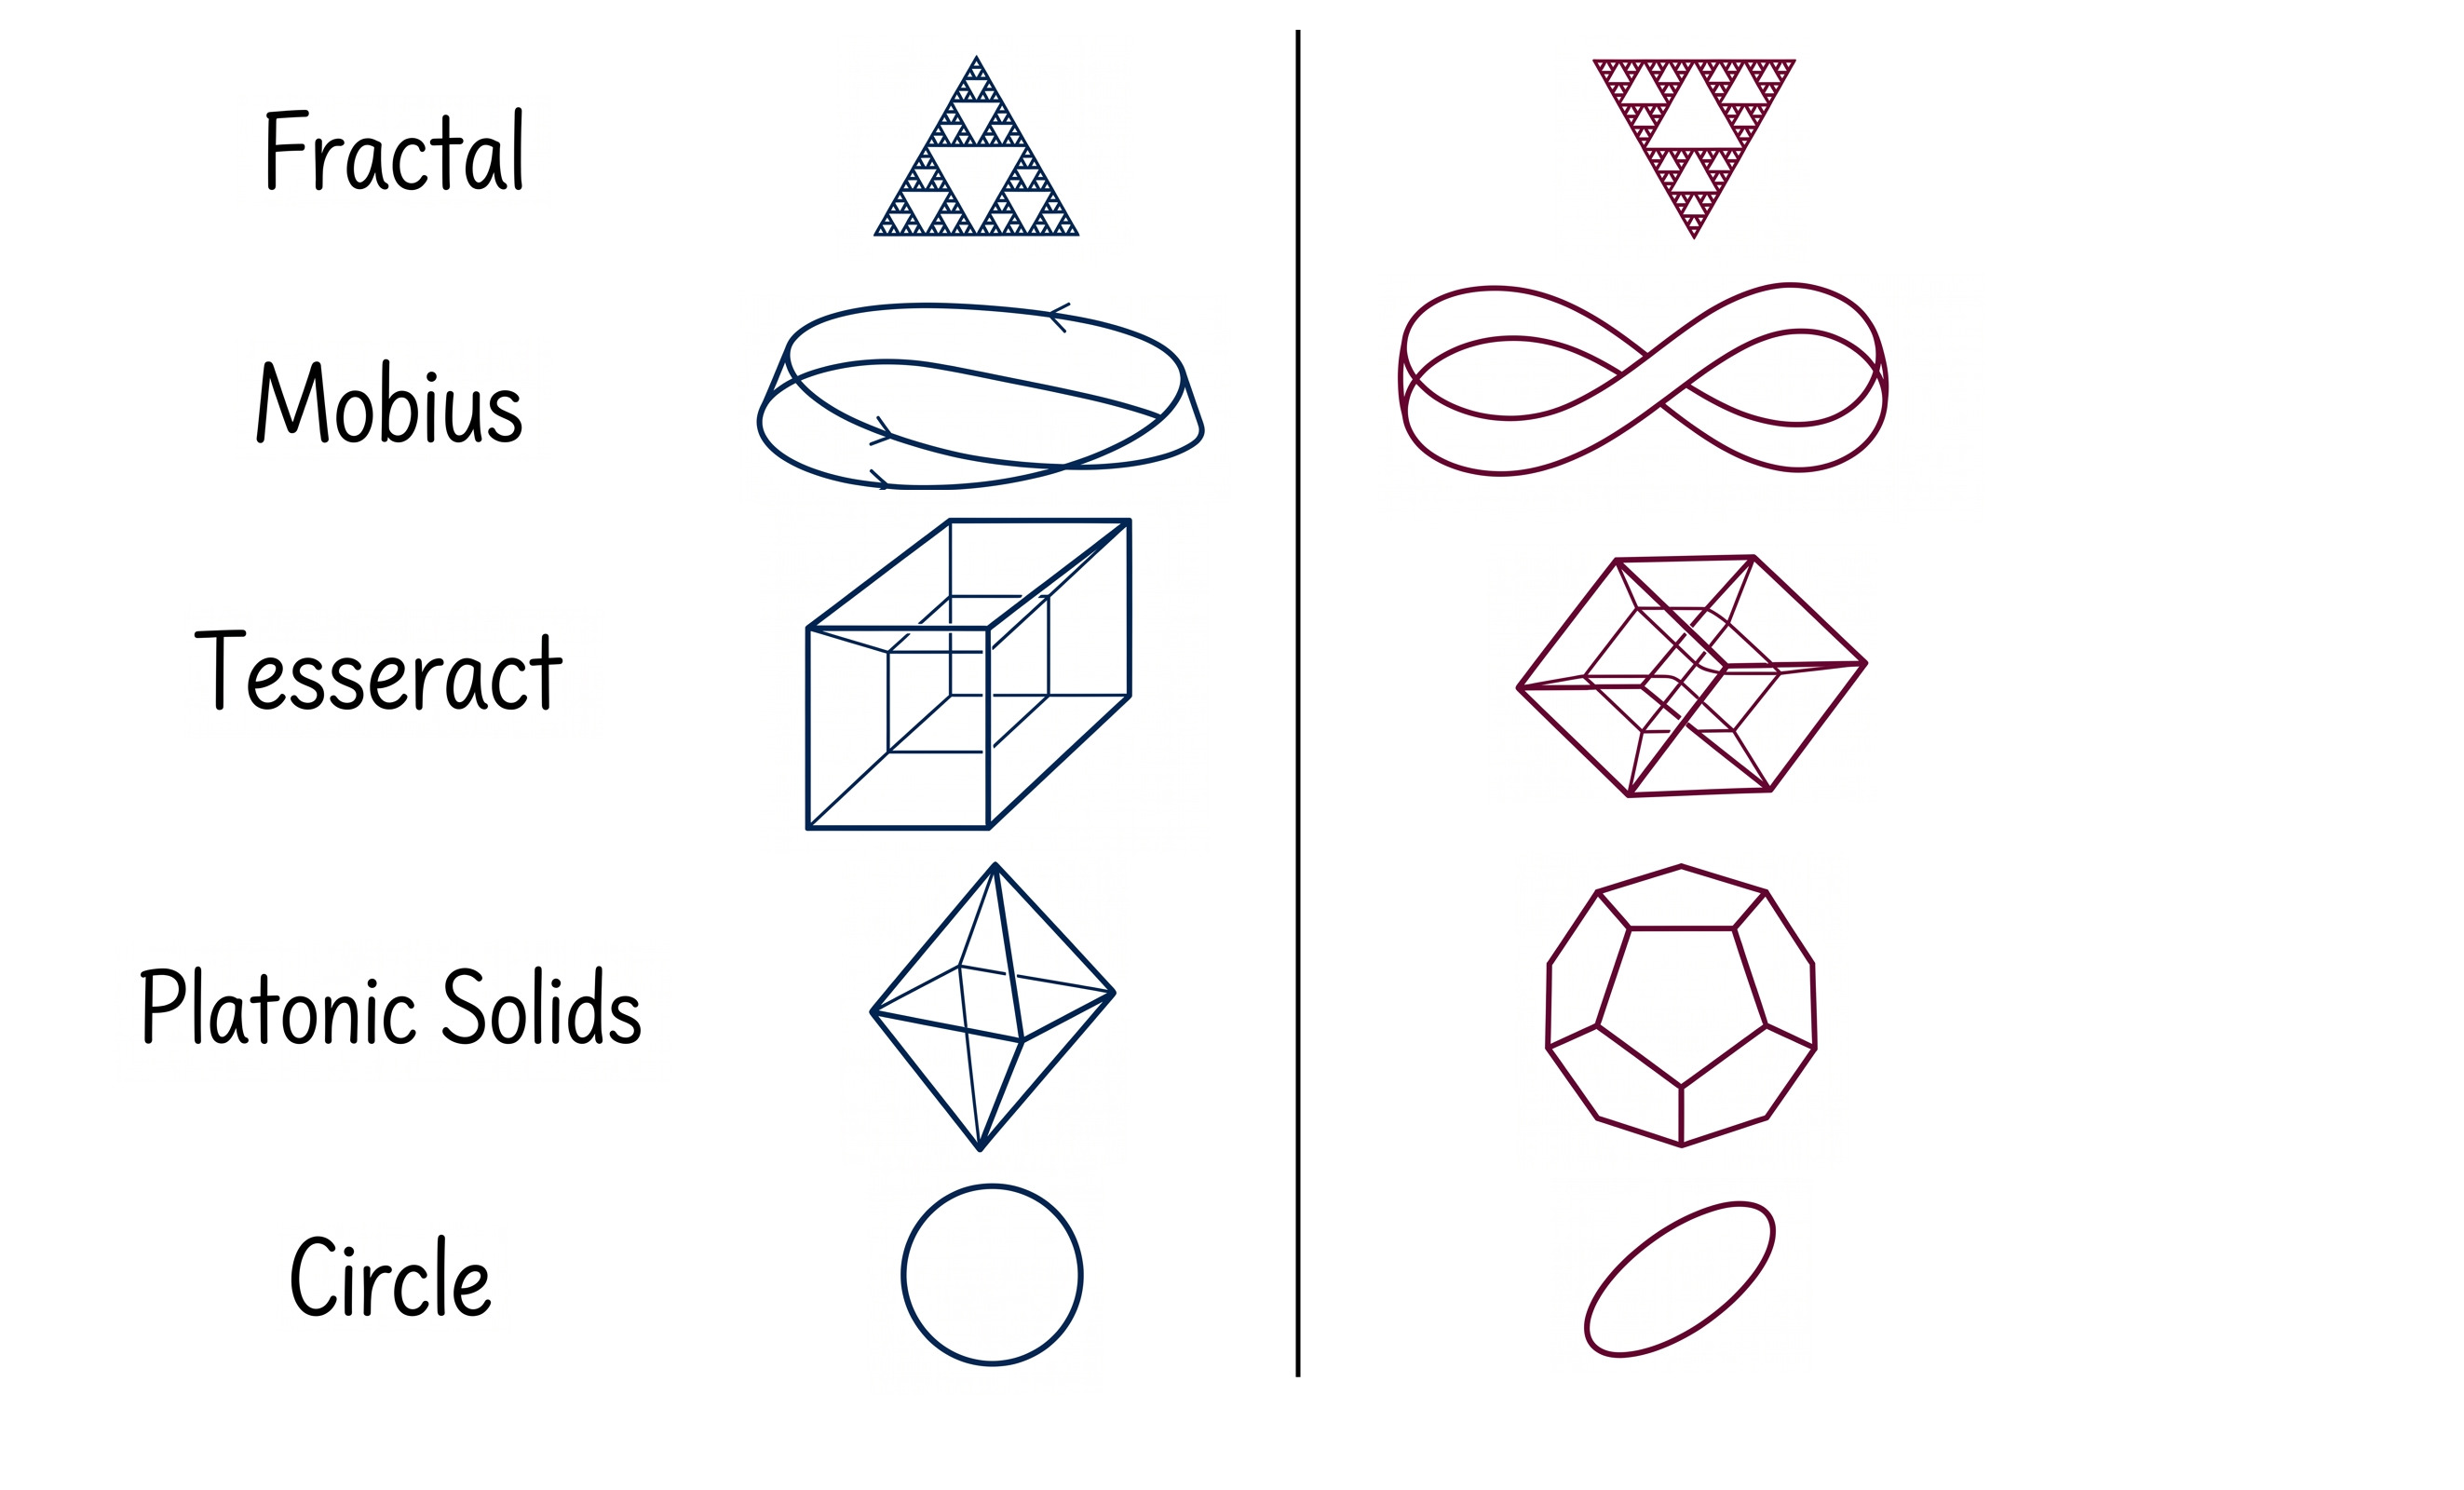
\includegraphics[width=0.8\textwidth]{../images/meta_learning_human.jpg}
    \caption{Hình minh họa một bài toán nhận diện hình học.}
    \label{fig:meta_learning_demos}
\end{figure}

Dựa trên cơ chế đó, \acrshort{maml} giải quyết bài toán \acrlong{fsl} thông qua một quá trình tối ưu gồm hai tầng (Hình \ref{fig:meta_learning_obj}). Với tầng lặp trong (inner loop), mô hình học xuất phát từ tham số khởi tạo chung $\theta_0$ thực hiện $T$ bước cập nhật gradient trên hàm mất mát tính trên tập hỗ trợ $S_i$ của tác vụ $\mathcal{T}_i$, theo phương trình \ref{eq:inner_loop}.
\begin{equation}
    \centering
    \phi_j = \phi_{j-1} - \alpha \nabla_{\phi} \mathcal{L}_{S_i}(\phi_{j-1}), \qquad j = 1, 2, \dots, T, \quad \phi{0} = \theta_0
    \label{eq:inner_loop}
\end{equation}
Trong đó $\alpha$ là tốc độ học của inner loop, và nghiệm sau $T$ bước được ký hiệu là $\phi_i^* := \phi_T$. Sau đó, ở tầng lặp ngoài (outer loop), tham số khởi tạo chung $\theta_0$ sẽ được cập nhật theo phương trình \ref{eq:outer_loop} sao cho tổng (hoặc trung bình) giá hàm mất mát trên các tập truy vấn $Q_i$, tính tại nghiệm đã thích ứng $\phi_i^*$, được tối thiểu hoá trên toàn bộ phân phối tác vụ.
\begin{equation}[h]
    \centering
    \theta = \theta_0 - \beta \nabla_\theta \sum_{k} \mathcal{L}_{Q_i}(\phi_i^*)
    \label{eq:outer_loop}
\end{equation}
Trong đó, $\beta$ là tốc độ học của outer loop, $\mathcal{L}_{Q_i}$ là hàm mất mát trên tập truy vấn $Q_i$ với mô hình sau khi cập nhật bởi inner loop và $\sum_{k}$ là tổng hàm mất mát của tất cả các tác vụ trong một meta-batch.

\begin{figure}[h]
    \centering
    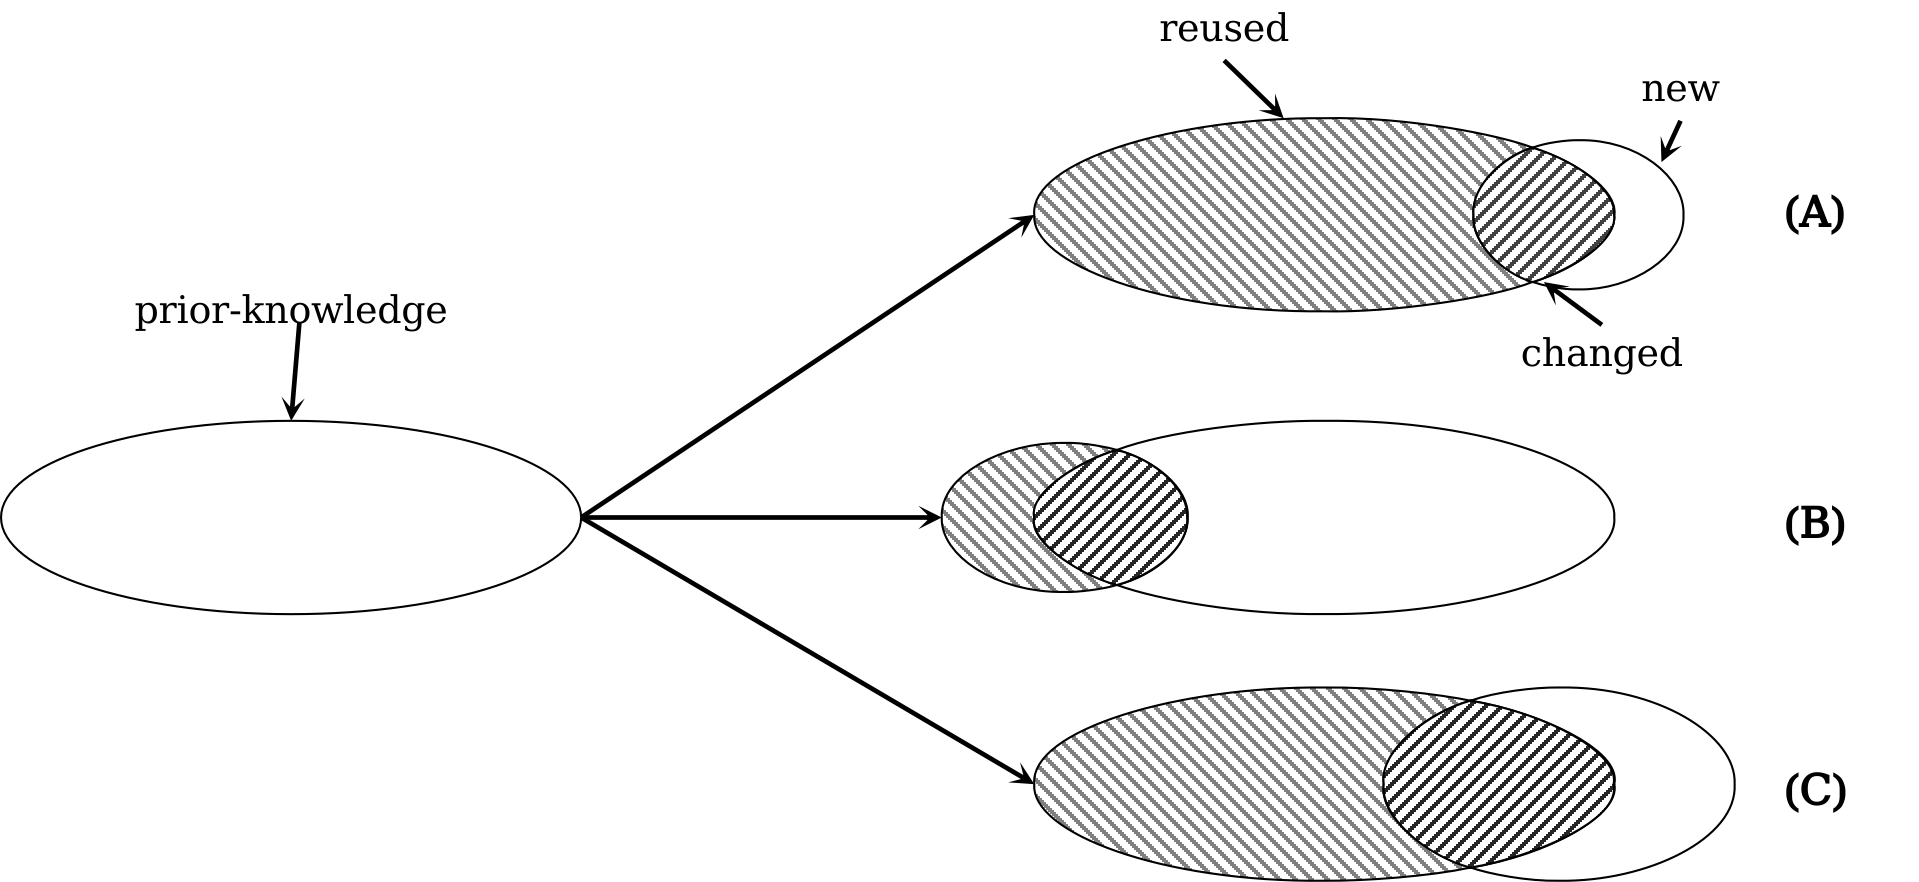
\includegraphics[width=0.8\textwidth]{../images/meta_learning_obj.png}
    \caption{Quá trình \acrshort{maml} tìm kiếm vị trí khởi tạo thuận lợi cho tham số $\theta_0$ trong giai đoạn meta-training.}
    \label{fig:meta_learning_process}
\end{figure}

Để lý giải cơ thích ứng nhanh của \acrshort{maml}, Raghu và các cộng sự \cite{raghu2019rapid} đã thực hiện thí nghiệm đóng băng phần thân trích xuất đặc trưng (backbone) $\theta_0^{b}$ và chỉ cho phép phần đầu phân loại (head) $\theta_0^{h}$ cập nhật trong inner loop - thuật toán ANIL (Almost No Inner Loop). Bằng cách so sánh biểu diễn của backbone trước và sau thích ứng thông qua CCA và CKA, nhóm tác giả cho thấy các lớp tích chập gần như không dịch chuyển, trong khi chỉ riêng head thay đổi đáng kể. Từ đó, đi tới kết luận rằng hiệu quả của \acrshort{maml} chủ yếu đến từ việc $\theta_0$ đã sẵn mang những đặc trưng tổng quát, có thể tái sử dụng nguyên trạng các đặc trưng này cho hầu hết tác vụ mới (feature reuse). Trạng thái này được khái quát hóa tại Hình \ref{fig:repr_space} A, trong đó không gian biểu diễn sau thích ứng ($\phi_i^*$) duy trì sự đồng nhất gần như tuyệt đối với không gian tiền nghiệm ($\theta_0$). Cũng đồng nghĩa với việc vai trò thực sự của $S_i$, trong trường hợp này, chỉ là căn chỉnh lại ranh giới quyết định ở phần đầu phân loại (head) cho phù hợp với từng tác vụ cụ thể.

Mặc dù vậy, giả thuyết về tính phổ quát của việc \emph{tái sử dụng đặc trưng (feature reuse)} bộc lộ sự hạn chế khi đối mặt với sự dịch chuyển phân phối (distribution shift) lớn giữa miền dữ liệu huấn luyện (meta-training) và miền kiểm tra (meta-testing). Oh và các cộng sự \cite{oh2020boil} đã phản bác hệ quả của ANIL thông qua một can thiệp kiến trúc đối xứng mang tên BOIL (Body Only Inner Loop) — chỉ cập nhật $\theta_0^{b}$ và đóng băng $\theta_0^{h}$. Kết quả là trên các môi trường có miền dữ liệu khác nhau (cross-domain), tri thức tiền nghiệm $\theta_0$ không chứa sẵn các biễu diễn có lợi và phù hợp cho tác vụ đích buộc phải dưới áp lực của $S_i$ dần bị thu hẹp và bị triệt tiêu tối đa, nhường chỗ cho sự dịch chuyển và hình thành các vùng biểu diễn hoàn toàn mới (Hình \ref{fig:repr_space} B). 

Từ sự đối lập của hai cơ chế trên, có thể thấy \acrshort{maml} tiêu chuẩn khi không bị ràng buộc bởi việc đóng băng trên toàn bộ mạng, đã cho phép nó hoạt động dựa trên một trạng thái linh hoạt điều chỉnh tỷ trọng giữa việc "tái sử dụng" và "tái cấu trúc". Lập luận này được củng cố bởi các thí nghiệm do Gou và các cộng sự thực hiện kiểm chứng trên các tập dữ liệu có sự khác biệt lớn, với kết luận tỷ trọng biến đổi của phần thân (backbone) tỷ lệ thuận với khoảng cách phân phối dữ liệu (domain shift). Hệ quả là, không gian biểu diễn chung $F$ của \acrshort{maml} sau khi thích ứng trở thành một môi trường giao thoa phức hợp bao gồm ba miền, (1) miền kế thừa nguyên trạng từ $\theta_0$, (2) miền đặc trưng cũ bị bẻ cong/điều biến dưới áp lực của $S_i$, và (3) miền tiếp thu các cấu trúc hoàn toàn mới (Hình \ref{fig:repr_space} C).

\begin{figure}[h]
    \centering
    
\includegraphics[width=\textwidth]{images/repr_space.png}
    \caption{Minh họa sự thay đổi của không gian biểu diễn $F$ sau thích ứng nhanh.}
    \label{fig:repr_space}
\end{figure}

\subsection{\acrfull{xai}}
\label{subsec:xai_bg}

Mặc dù \acrshort{maml} và các biến thể đã chứng minh được hiệu quả trong việc cải thiện \emph{phương thức} thích ứng, cơ chế vận hành của "lực định hướng" này tại cấp độ đặc trưng vẫn là một dạng "hộp đen". Các phương pháp hiện nay chưa cung cấp một lý giải tường minh cho câu hỏi: \textit{Tại sao một tập hỗ trợ cụ thể lại điều hướng mô hình tới một hướng thích ứng nhất định?} Sự thiếu vắng này đặc biệt đáng chú ý tại không gian đặc trưng chung $F$. Dẫn đến việc chúng ta không thể truy vết được nguồn gốc của các tương quan giả khi mô hình rơi vào trạng thái chuyển giao tiêu cực (negative transfer).

\textbf{\acrfull{xai}} là lĩnh vực nghiên cứu các phương pháp giúp con người hiểu được cơ chế ra quyết định của một mô hình học máy, ra đời như một phản ứng tất yếu trước sự phát triển của các mô hình học sâu. Trong khi các mô hình như hồi quy tuyến tính hay cây quyết định vốn có tính minh bạch nội tại (intrinsic model), cho phép truy vết trực tiếp đường đi từ đặc trưng đầu vào đến dự đoán đầu ra, thì các kiến trúc phức tạp hơn như mạng nơ-ron sâu lại đánh đổi tính minh bạch đó để lấy độ chính xác, trở thành những mô hình "hộp đen" mà cơ chế nội tại không thể quan sát trực tiếp.

Dựa trên thời điểm can thiệp vào mô hình, các kỹ thuật \acrshort{xai} được chia thành hai nhóm. \emph{Ante-hoc}, với tính khả diễn giải được tích hợp ngay từ khi thiết kế kiến trúc mô hình (cây quyết định, cơ chế attention, Self-Explaining Neural Networks) và \emph{post-hoc}, với các kỹ thuật diễn giải được áp dụng ngay sau khi mô hình đã huấn luyện xong, nhằm phân tích và diễn giải một mô hình đã có mà không cần huấn luyện lại. Do các phương pháp post-hoc không yêu cầu thay đổi kiến trúc hay quy trình huấn luyện gốc của mô hình, nên chúng có tính linh hoạt cao và có thể áp dụng cho các mô hình hộp đen phức tạp đã được huấn luyện. Theo Arrieta và các cộng sự \cite{arrieta2020explainable}, các kỹ thuật post-hoc thường dựa trên một trong ba cách tiếp cận chính. Gồm, đơn giản hoá mô hình (model simplification, xây dựng một mô hình thay thế — surrogate — dễ diễn giải hơn để xấp xỉ hành vi cục bộ của mô hình hộp đen, như LIME), độ liên quan đặc trưng (feature relevance explanation, xếp hạng mức độ quan trọng của từng đặc trưng đầu vào đối với một dự đoán cụ thể, như SHAP) và cuối cùng là trực quan hoá (visual explanation, cho phép con người quan sát trực tiếp bằng hình ảnh cơ chế mà mô hình đưa ra quyết định).

Trong ba hướng trên, trực quan hoá cho phép con người dễ dàng diễn giải lựa chọn của mô hình thông qua hình ảnh trực quan thay vì các con số trừu tượng. Tiêu biểu đối với các mạng nơ-ron tích chập (CNN) dùng cho các bài toán thị giác máy tính, các kỹ thuật trực quan hoá mức độ đóng góp (attribution visualization) đã được phát triển nhằm định vị và làm nổi bật những vùng đầu vào chi phối mạnh nhất đến kết quả dự đoán của mô hình. Khởi nguồn cho hướng tiếp cận này là bản đồ nổi bật (saliency map) của Simonyan và các cộng sự \cite{simonyan2014visualising}, sử dụng đạo hàm điểm ảnh (vanilla gradient) ứng với một lớp mục tiêu để sinh ra bản đồ có cùng kích thước không gian với ảnh đầu vào, qua đó định lượng trực tiếp mức độ đóng góp của từng vị trí vào quyết định của mô hình. Kế thừa nền tảng này, Guided Backpropagation \cite{springenberg2014striving} sau đó đã điều chỉnh lại quy tắc lan truyền ngược qua hàm kích hoạt ReLU nhằm triệt tiêu các gradient âm, từ đó tạo ra bản đồ phân bổ sắc nét hơn, dù vẫn bị giới hạn ở các điểm ảnh riêng lẻ. Nhằm dịch chuyển trọng tâm phân tích sang các vùng không gian ngữ nghĩa, Zhou và các cộng sự \cite{zhou2016learning} đề xuất Class Activation Mapping (CAM) bằng cách chèn thêm lớp global average pooling vào cuối kiến trúc mạng. Tuy nhiên, đổi lại CAM đòi hỏi phải thay đổi kiến trúc gốc và huấn luyện lại mô hình. Để khắc phục điểm nghẽn này, Gradient-weighted Class Activation Mapping (Grad-CAM) \cite{selvaraju2020grad} đã tổng quát hoá CAM, cho phép áp dụng hậu diễn giải (post-hoc) trên mọi mạng CNN mà không cần can thiệp kiến trúc. Bằng cách tận dụng gradient của lớp mục tiêu lan truyền ngược đến lớp tích chập cuối cùng, Grad-CAM đã tổng hợp thành một bản đồ nhiệt không gian, một đặc tính vô cùng giá trị khi làm việc với các mô hình đã huấn luyện sẵn. Mặc dù vậy, một điểm mù cố hữu của toàn bộ các biến thể CAM là việc trích xuất tín hiệu diễn giải luôn bị bó hẹp tại một \emph{trạng thái tham số tĩnh} duy nhất, tức thời điểm suy luận sau khi mạng đã hội tụ. Đặc tính tĩnh này khiến chúng trở nên bất lực khi phải giải phẫu hệ động lực học của quá trình thích ứng nhanh (fast adaptation), nơi không gian biểu diễn không đứng yên mà liên tục biến thiên qua từng bước cập nhật gradient.

\subsection{Correctness và trustworthiness của một phương pháp XAI}

Theo Hướng dẫn Đạo đức cho AI Đáng tin cậy (Ethics Guidelines for Trustworthy AI) của Nhóm chuyên gia cấp cao về AI thuộc Ủy ban Châu Âu (EC) \cite{eu2019trustworthy}, tính minh bạch (transparency), bao hàm khả năng diễn giải (explainability), là một trong bảy yêu cầu tiên quyết để kiến tạo một hệ thống AI đáng tin cậy (\emph{trustworthy}). Dẫu vậy, cần phân định rạch ròi giữa hai cấp độ khái niệm: "đáng tin cậy" là thuộc tính vĩ mô của \emph{toàn bộ hệ thống}, trong khi một phương pháp XAI, để đóng góp vào thuộc tính này, trước hết phải tự chứng minh được \textbf{tính đúng đắn} (\emph{correctness}) nội tại. Cụ thể, điều này đòi hỏi mức độ trung thành (\emph{faithfulness}) tuyệt đối của lời giải thích đối với cơ chế ra quyết định thực tế của mô hình, hoàn toàn độc lập với việc lời giải thích đó "nhìn có vẻ hợp lý" dưới lăng kính trực giác cảm quan của con người.

Để định lượng tính trung thành này, \textbf{nguyên lý thứ nhất} được thiết lập dựa trên kỹ thuật nhiễu loạn đặc trưng, nổi bật là phép kiểm định \emph{xóa-và-đo} (deletion test) do Samek và các cộng sự \cite{samek2016evaluating} đặt nền móng. Với ý tưởng cốt lõi là nếu bản đồ phân bổ định vị chuẩn xác các vùng đầu vào mang tính quyết định, thì việc tuần tự che khuất các vùng này (bằng nhiễu hoặc giá trị nền) theo thứ tự độ quan trọng giảm dần sẽ khiến hiệu năng dự đoán của mô hình suy sụp nhanh hơn đáng kể so với việc xóa ngẫu nhiên. Kế thừa tư tưởng này, Petsiuk và các cộng sự \cite{petsiuk2018rise} đã tiêu chuẩn hóa thành hai độ đo nghịch đảo — \emph{Xóa (Deletion)} và \emph{Thêm (Insertion)} — cho phép đánh giá khách quan tính trung thành thông qua diện tích dưới đường cong (AUC) của biểu đồ hiệu năng, qua đó triệt tiêu hoàn toàn sự phụ thuộc vào sự phán xét chủ quan của mắt người.

\textbf{Nguyên lý thứ hai}, được biết đến qua các phép kiểm tra tính hợp lý (sanity checks) do Adebayo và các cộng sự \cite{adebayo2018sanity} đề xuất, lại tập trung vào khả năng phản chiếu tri thức. Nguyên lý này lập luận, "một bản đồ phân bổ đích thực phải thể hiện sự \emph{nhạy cảm} trước những biến động phá vỡ cấu trúc tri thức tiềm ẩn của mạng". Thông qua kỹ thuật ngẫu nhiên hóa tham số lan truyền ngược từ lớp đầu ra (\emph{cascading randomization}), nhóm tác giả chỉ ra việc nếu bản đồ phân bổ gần như bất biến dù trọng số mô hình đã bị phá hủy ngẫu nhiên, phương pháp \acrshort{xai} đó thực chất không trích xuất bất kỳ tri thức nào, mà chỉ đang hoạt động như một bộ dò biên cạnh (edge detector) vô tri. Nghiên cứu này đã phơi bày một lỗ hổng nghiêm trọng của nhiều phương pháp \acrshort{xai} phổ biến thời bấy giờ (như Guided Backpropagation) khi chúng hoàn toàn trơ lỳ trước các lớp trọng số bậc cao, một "tử huyệt" bị che đậy đằng sau hình thức trực quan bắt mắt.

Tuy nhiên, như đã phân tích trước đó, dù cả hai nguyên lý trên đều cung cấp một khung đánh giá vững chắc, nhưng cũng đều tồn tại một điểm mù cố hữu. Chúng được thiết kế độc quyền cho các kiến trúc mô hình \emph{tĩnh}, nơi tín hiệu diễn giải được trích xuất từ một trạng thái tham số bất động tại một thời điểm suy luận duy nhất. Khi áp đặt vào hệ động lực học của quá trình thích ứng nhanh (fast-adaptation), nơi các bản đồ phân bổ được trích xuất liên tục chạy dọc theo một quỹ đạo cập nhật gradient, tính hiệu lực của các nguyên lý này lập tức bị thách thức. Bài toán làm thế nào để định lượng tính trung thành của một diễn giải XAI không chỉ tại một tọa độ tĩnh, mà xuyên suốt \emph{một chuỗi các biến thiên tham số liên tiếp}, hiện vẫn là một "vùng tối" chưa có lời giải trong cộng đồng nghiên cứu, đòi hỏi một nỗ lực tái định chuẩn và mở rộng hệ thống đo lường toàn diện.

\section{Các nghiên cứu liên quan}

Dựa trên nền tảng lý thuyết ở Mục~\ref{sec:background}, chúng tôi tiến hành rà soát bốn nhóm nghiên cứu liên quan trực tiếp đến đề tài. Gồm, các phương pháp hiện có giải quyết bài toán tác vụ không đồng nhất (heterogenous task) và hiện tượng Negative Transfer (Mục \ref{subsec:negative_transfer}), các công cụ hiện có cho hậu diễn giải (post-hoc) tổng quát dựa trên gradient và nhiễu loạn (perturbation) (Mục \ref{subsec:background_post_hoc}), khảo sát các phương pháp diễn giải hiện đang áp dụng riêng cho meta-learning (Mục \ref{subsec:xai_metalearning}) và attribution dựa trên quỹ đạo tham số (Mục \ref{subsec:trajectory_attribution}). Mục~\ref{subsec:relatedwork_synthesis} tổng hợp lại toàn bộ và chỉ ra các khoảng trống còn tồn tại.

\subsection{Tác vụ không đồng nhất (heterogeneous task) và hiện tượng Negative Transfer}
\label{subsec:negative_transfer}

Phần lớn các phương pháp meta-learning giả định ngầm rằng tập hợp tác vụ dùng để meta-training tương đối đồng nhất (\emph{homogeneous}), sao cho một điểm khởi tạo chung $\theta_0$ duy nhất là đủ tốt cho mọi tác vụ \cite{finn2017model, snell2017prototypical, vinyals2016matching, santoro2016meta}. Một nhánh nghiên cứu song song đã chỉ ra giả định này thường bị vi phạm trong thực tế, khi các tác vụ đích đến từ phân phối tác vụ không đồng nhất (task heterogenous) với phân phối tác vụ trong giai đoạn meta-training. Dẫn đến sự ra đời của các cơ chế tùy chỉnh (customize) tri thức tiên nghiệm theo từng cụm hoặc nhóm tác vụ thay vì chia sẻ toàn cục.

Yao và các cộng sự đã đề xuất \acrfull{hsml} \cite{yao2019hierarchically}, tổ chức các tác vụ thành một cấu trúc phân cụm phân cấp, qua đó đặc thù hóa tri thức chuyển giao cho từng nhóm tác vụ thay vì buộc mọi tác vụ chia sẻ một tri thức toàn cục, dựa trên cảm hứng từ cách con người tổ chức tri thức theo thứ bậc. Tiếp nối hướng đi này, nhóm tác giả tiếp tục phát triển \acrfull{arml} \cite{yao2020automated}, thay thế cho cấu trúc phân cụm thủ công bằng một siêu đồ thị tri thức (meta-knowledge graph) được xây dựng một cách tự động, cho phép mô hình hóa quan hệ giữa các tác vụ linh hoạt hơn. Theo đó, một hướng tiếp cận khác, HetMAML do Chen và các cộng sự \cite{chen2021hetmaml} đã mở rộng bài toán tác vụ không đồng nhất sang không gian đặc trưng đầu vào (heterogeneous input/modality), làm rõ tính đa dạng của khái niệm "tác vụ không đồng nhất", từ sự không đồng nhất về phân phối ngữ nghĩa đến không đồng nhất về cấu trúc dữ liệu đầu vào.

Ở một góc nhìn khác, Yue và các cộng sự tập trung vào nguyên nhân nhân quả thay vì cấu trúc tác vụ, và đề xuất phương pháp \acrfull{ifsl} \cite{yue2020interventional} nhằm tạo ra sự can thiệp nhân quả để khác phục hiện tượng chuyển giao tiêu cực (negative transfer). Đồng thời, lý giải hiện tượng này thông qua một mô hình cấu trúc nhân quả (Structural Causal Model), trong đó tri thức tiền huấn luyện đóng vai trò như một biến gây nhiễu (confounder) và tạo ra các tương quan giả cho việc dự đoán nhãn, khiến mô hình vô tình gây ra sai lệch. Song song đó, Deleu và Bengio \cite{deleu2018negative} định nghĩa khái niệm \emph{negative adaptation}: vì MAML chỉ tối thiểu hóa hàm mất mát trên tập truy vấn mà không có ràng buộc chặt chẽ, do đó tham số sau thích ứng có thể làm giảm hiệu năng so với trạng thái khởi tạo $\theta_0$

Gần đây, Si và các cộng sự đề xuất phương pháp \acrfull{hetero} \cite{si2025meta}, nhằm giải quyết bài toán từ góc độ \emph{độ khó không đồng đều} giữa các tác vụ. Thay vì gán trọng số bằng nhau cho toàn bộ các tác vụ trong giai đoạn meta-training như giả định của \acrshort{maml}, \acrshort{hetero} sử dụng mục tiêu học tập dựa tên xếp hạng (rank-based task-level learning objective) để ngăn các tác vụ "dễ" lấn át quá trình tối ưu. Đồng thời, Parast và các cộng sự cũng đề xuất \acrfull{hsfm} \cite{parast2026hsfm} nhằm can thiệp trực tiếp lên các biểu diễn, bằng cách trực tiếp thao tác trên các embedding của tập hỗ trợ trong không gian đặc trưng đã đóng băng (frozen backbone), lan truyền ngược qua các bước thích ứng của bộ phân loại để tinh chỉnh support embeddings, giúp mô hình hoạt động tốt hơn trước các tương quan giả.

Nhìn chung, các nghiên cứu giải quyết bài toán tác vụ không đồng nhất cho thấy một xu hướng nhất quán. Cộng đồng ngày càng thừa nhận tính không đồng nhất là nguyên nhân cốt lõi gây suy giảm hiệu năng thích ứng, và các giải pháp đang đi sâu vào can thiệp ở cấp độ biểu diễn (embeddings). Tuy nhiên, không một phương pháp nào trong chuỗi này hướng đến việc \emph{diễn giải tường minh} cơ chế mà $S_i$ đã định hướng sai ở đâu trong không gian đặc trưng chung. Tất cả các nghiên cứu hiện hành đều dừng lại ở mức phát hiện qua biểu hiện của các chỉ số (thường là độ chính xác suy giảm) hoặc sửa chữa qua tối ưu hóa lại biểu diễn, mà chưa cung cấp một bản đồ phân bổ (attribution) trực quan nào có thể chẩn đoán được nguyên nhân của sự chệch hướng trong quá trình thích ứng.

\subsection{Các phương pháp giải thích hậu nghiệm dựa trên gradients và nhiễu loạn}
\label{subsec:background_post_hoc}

Ngoài các kiến trúc diễn giải nội tại như Class Activation Mapping đã trình bày ở Mục~\ref{subsec:xai_bg}, cộng đồng nghiên cứu XAI đã phát triển các phương pháp \textbf{hậu diễn giải} (\emph{post-hoc}) tổng quát. Các kỹ thuật này không bị giới hạn bởi cấu trúc kiến trúc mạng cụ thể, cho phép phân tích hành vi của mô hình một cách linh hoạt hơn. Có thể chia các phương pháp này thành hai nhánh chính dựa trên cơ chế tác động.

Nhánh thứ nhất dựa trên phân tích gradient (đạo hàm) của đầu ra theo từng đặc trưng đầu vào. Integrated Gradients \cite{sundararajan2017axiomatic} tích phân gradient dọc theo đường thẳng nối giữa một điểm nền (\emph{baseline}) và dữ liệu cần giải thích, thoả mãn các tiên đề về \emph{Sensitivity} và \emph{Implementation Invariance}. Trong khi đó, SmoothGrad \cite{smilkov2017smoothgrad} khắc phục tình trạng nhiễu bằng cách lấy trung bình các bản đồ gradient được tính trên các biến thể của dữ liệu gốc đã bị thêm nhiễu ngẫu nhiên, dựa trên quan sát rằng gradient của các mô hình sâu thường dao động mạnh trong vùng lân cận nhỏ của đầu vào.

Nhánh thứ hai dựa trên kỹ thuật \textbf{nhiễu loạn} (\emph{perturbation}), nơi tầm quan trọng của đặc trưng được suy luận qua sự biến thiên của đầu ra khi dữ liệu đầu vào bị thay đổi thông qua làm nhiễu hoặc xáo trộn. \acrfull{lime} \cite{ribeiro2016lime} xấp xỉ hành vi cục bộ của mô hình "hộp đen" bằng một mô hình tuyến tính đơn giản, huấn luyện trên tập các mẫu bị nhiễu loạn xung quanh điểm dữ liệu mục tiêu. \acrfull{shap} \cite{lundberg2017unified} định lượng đóng góp của đặc trưng dựa trên giá trị Shapley, đảm bảo tính công bằng (\emph{efficiency, symmetry}) mà các phương pháp như LIME không đạt được. RISE \cite{petsiuk2018rise} tạo bản đồ phân bổ được trích xuất từ sự tương quan giữa các mặt nạ ngẫu nhiên che đi dữ liệu đầu vào và điểm số dự đoán tương ứng.

Tuy nhiên, điểm chung của toàn bộ các phương pháp kể trên là bất kể dựa trên gradient hay nhiễu loạn, chúng đều giải thích hành vi của mô hình dựa trên giả định về một \emph{trạng thái tham số tĩnh}. Các phương pháp này được thiết kế để giải thích hành vi mô hình tại một thời điểm suy luận duy nhất, do đó hoàn toàn thiếu khả năng tích lũy hoặc tổng hợp thông tin dọc theo một quỹ đạo biến thiên tham số. Đây chính là rào cản mang tính hệ thống khiến chúng không thể triển khai nhằm diễn giải cơ chế thích ứng nhanh của các phương pháp dựa trên gradient. 

\subsection{Các phương pháp XAI cho Meta-Learning và Few-Shot Learning}
\label{subsec:xai_metalearning}

Mặc dù các nỗ lực giải quyết bài toán tác vụ không đồng nhất nói riêng và việc khai mở bản chất "hộp đen" của meta-learning nói chung đã đạt được những bước tiến nhất định, nhưng, nhìn chung việc xây dựng các khung diễn giải toàn diện và hệ thống vẫn còn nhiều hạn chế. Thực tế, các hướng nghiên cứu hiện nay vẫn tồn tại sự phân hóa rõ rệt, các nỗ lực diễn giải đang tập trung vào những hướng đi rất khác biệt thay vì hội tụ về một phương pháp chung. Cụ thể, có thể phân loại hai hướng tiếp cận tiêu biểu gần đây trong việc nỗ lực diễn giải cơ chế hoạt động của các mô hình meta-learning.

\textbf{Hướng thứ nhất} mở rộng \textit{influence functions}, công cụ vốn được thiết kế để định lượng giá trị ảnh hưởng của một mẫu dữ liệu huấn luyện lên dự đoán của mô hình, sang cấu trúc phù hợp với bối cảnh meta-learning. Đại diện tiêu biểu là TLXML \cite{mitsuka2025tlxml}, phương pháp này định lượng mức độ ảnh hưởng của từng \textit{tác vụ} trong giai đoạn meta-training lên hành vi thích ứng trên một tác vụ đích. Bằng cách sử dụng xấp xỉ Gauss-Newton cho Hessian, TLXML giải quyết được bài toán chi phí tính toán cao vốn là rào cản đặc thù của \textit{influence functions} trong bối cảnh tối ưu hóa hai tầng. Tuy nhiên, phương pháp này vẫn coi thao tác thích ứng trên tập hỗ trợ ($S_i$) là một "hộp đen" ở cấp độ tác vụ, đồng thời đòi hỏi quyền truy cập vào toàn bộ dữ liệu đã huấn luyện trong quá trình meta-training, một điều kiện khó đáp ứng trong triển khai thực tế.

\textbf{Hướng thứ hai} tích hợp trực tiếp các kỹ thuật dựa trên CAM vào quy trình huấn luyện few-shot nhằm giám sát mô hình tập trung vào đặc trưng ngữ nghĩa thay vì tương quan giả. Một số framework như \textit{expert-guided} cho ảnh y khoa \cite{uddin2025expert} là đại diện sử dụng hướng đi này, bằng cách sử dụng Grad-CAM kết hợp với hàm mất mát căn chỉnh (alignment loss) giữa bản đồ nhiệt (heat map) và vùng chú thích đã được chuyên gia tạo sẵn (ground-truth). Do đó, điểm hạn chế chung của các phương pháp này là bản đồ nhiệt chỉ được trích xuất tại thời điểm mô hình \textit{đã thích ứng hoàn tất} ($f_{\phi_i^*}$) tức là chỉ diễn giải kết quả suy luận cuối cùng và chúng cần các vùng chú thích được tạo sẵn. Thành thử, các phương pháp này hoàn toàn bỏ qua việc giải thích bản chất của quá trình dịch chuyển tham số từ điểm khởi tạo $\theta_0$ sang trạng thái thích ứng $\phi_i^*$.

Tóm lại, cả hai hướng tiếp cận trên, dù có khác biệt về mặt kỹ thuật, nhưng đều bộc lộ giới hạn chung về mặt diễn giải. Với hướng thứ nhất bỏ qua cơ chế thích ứng nội tại ở cấp độ đặc trưng, trong khi hướng thứ hai xem nhẹ vai trò định hướng của tập hỗ trợ trong chính bước dịch chuyển không gian tham số.

\subsection{Attribution dựa trên quỹ đạo huấn luyện}
\label{subsec:trajectory_attribution}

Khác với các tiến trình huấn luyện cố định, quá trình thích ứng nhanh (\textit{fast adaptation}) trong meta-testing được đặc trưng bởi một chuỗi cập nhật tham số liên tiếp (như mô tả tại Phương trình \ref{eq:inner_loop}). Đặc tính này này đòi hỏi một cơ chế diễn giải mới cho các công cụ giải thích. Thay vì tìm kiếm nguyên nhân tại một trạng thái dừng (\textit{static state}), ta cần một cơ chế có khả năng truy vết sự đóng góp của dữ liệu xuyên suốt toàn bộ \textbf{quỹ đạo biến thiên tham số} (\textit{parameter trajectory}). Để xác lập cơ sở lý thuyết cho phương pháp đề xuất, chúng tôi sẽ hệ thống hóa các hướng nghiên cứu attribution hiện nay.

\textbf{Influence Functions} được Koh và các cộng sự \cite{koh2017understanding} lần đầu đưa ra khái niệm xuất phát từ thống kê bền vững (robust statistics) áp dụng vào học máy, nhằm  ước lượng ảnh hưởng của mẫu huấn luyện $z_i$ lên loss tại mẫu kiểm thử $z_{\text{test}}$ thông qua khai triển Taylor bậc nhất.
\begin{equation}
\mathcal{I}{\text{up,loss}}(z_i, z{\text{test}}) = -\nabla_\theta \mathcal{L}(z_{\text{test}}, \hat\theta)^\top H_{\hat\theta}^{-1} \nabla_\theta \mathcal{L}(z_i, \hat\theta).
\end{equation}

Phương pháp này chỉ quan sát \emph{trạng thái hội tụ} $\hat{\theta}$, đòi hỏi mô hình khả vi bậc hai, lồi chặt và chi phí tính toán nghịch đảo Hessian $O(np^2+p^3)$ rất lớn.

\textbf{Representer Point Selection} được Yeh và cộng sự \cite{yeh2018representer} giới thiệu dựa trên định lý representer cho tầng cuối của mạng nơ-ron. Với điều kiện chính quy hoá $L_2$ trên trọng số $\Theta_1$ của tầng cuối, giá trị tiền kích hoạt (pre-activation) tại một điểm kiểm thử $x_t$ có thể được phân tích thành tổ hợp tuyến tính của các đặc trưng huấn luyện.

\begin{equation}
    \Phi(x_t, \Theta^*) = \sum_{i=1}^n \alpha_i f_i^\top f_t, \qquad \alpha_i = \frac{1}{-2\lambda n}\frac{\partial \mathcal{L}(x_i, y_i, \Theta)}{\partial \Phi(x_i, \Theta)}.
\end{equation}

Phương pháp này tách biệt đóng góp \emph{kích thích} ($\alpha_i > 0$) và \emph{ức chế} ($\alpha_i < 0$), đồng thời hiệu quả hơn Influence Functions nhờ tránh được Hessian. Tuy nhiên, nó vẫn bị giới hạn tại \emph{điểm dừng tĩnh} $\Theta^*$ và chỉ giải thích được logit dự đoán, không trực tiếp giải thích được loss.

\textbf{TracIn (Attribution dựa trên quỹ đạo)} được Pruthi và các cộng sự \cite{pruthi2020estimating} đưa ra nhằm giải quyết các hạn chế của hai phương pháp trên. Đồng thời cũng là phương pháp duy nhất định lượng ảnh hưởng thông qua tích lũy gradient dọc theo quỹ đạo huấn luyện.
\begin{equation}
\mathcal{I}(z_i, z_{\text{test}}) = \sum_{e=1}^{E} \nabla_{\theta} \mathcal{L}(z_i, \theta_e) \cdot \nabla_{\theta} \mathcal{L}(z_{\text{test}}, \theta_e).
\label{eq:trajectory_attribution}
\end{equation}
Trực giác cốt lõi của TracIn là xấp xỉ tổng mức giảm loss trên mẫu kiểm thử, tích luỹ qua toàn bộ quá trình huấn luyện, mỗi khi mẫu huấn luyện $z_i$ được sử dụng để cập nhật tham số. Về bản chất, đây là một phép tích luỹ (aggregation) tín hiệu attribution qua \emph{nhiều trạng thái tham số liên tiếp} $\{\theta_e\}_{e=1}^{E}$, thay vì chỉ tại một trạng thái duy nhất như hai phương pháp ở trên. Nhờ vậy, TracIn không đòi hỏi điều kiện hội tụ hay tối ưu bậc nhất, và có thể áp dụng cho bất kỳ mô hình nào huấn luyện bằng SGD hoặc biến thể của nó.

\subsection{Tổng hợp và định vị nghiên cứu}
\label{subsec:relatedwork_synthesis}

Từ các cơ sở lý thuyết và phân tích ở trên, ta có thể nhận thấy ba khoảng trống nổi bật khi đối chiếu chúng với nhau. \textbf{Thứ nhất}, các phương pháp diễn giải cho meta-learning hiện có (TLXML, Grad-CAM-FSL) đều xử lý thao tác thích ứng ở một trong hai cách, hoặc là diễn giải hộp đen ở cấp tác vụ, hoặc là chỉ quan sát tại trạng thái cuối cùng và vẫn chưa tồn tại phương pháp nào tổng hợp các phân bổ (attribution) qua nhiều trạng thái tham số của chính quá trình thích ứng nhanh (fast-adaptation). \textbf{Thứ hai}, toàn bộ các phương pháp giải quyết không đồng nhất/negative transfer (HSML, ARML, IFSL, HeTRoM, HSFM) đều dừng ở mức biểu hiện (đo bằng hiệu năng, như HSML/ARML/HeTRoM) hoặc sửa chữa (chỉnh sửa biểu diễn, như \acrshort{ifsl} hoặc \acrshort{hsfm}), trong đó \acrshort{hsfm} là phương pháp duy nhất thao tác đa trạng thái trong không gian đặc trưng, nhưng mục tiêu của nó vẫn là sửa chữa để tăng hiệu năng, không phải sinh ra một attribution có thể diễn giải được cho con người. \textbf{Thứ ba}, các phương pháp giải thích dựa trên việc truy vết quỹ đạo như TracIn chứng minh nguyên lý tích luỹ attribution qua nhiều trạng thái tham số là một hướng đi vững chắc về mặt toán học, nhưng chỉ được xây dựng cho bối cảnh huấn luyện dài hạn nhằm quy kết trách nhiệm cho từng mẫu dữ liệu huấn luyện, không phải cho bối cảnh thích ứng nhanh của meta-learning. \textbf{Cuối cùng,} chưa có phương pháp nào kết hợp đồng thời cả ba đặc điểm, diễn giải được cho con người, tổng hợp thông tin qua toàn bộ $T$ bước của quá trình thích ứng thay vì một trạng thái đơn lẻ, và không đòi hỏi quyền truy cập vào tập dữ liệu meta-training.


%\section{Quy định chung}

%Báo cáo phải được trình bày ngắn gọn, rõ ràng, mạch lạc, sạch sẽ, không được tẩy xóa, có đánh số trang, đánh số bảng biểu, hình vẽ, đồ thị. 

%Nội dung báo cáo được phân thành các chương. Số thứ tự của các chương, mục được đánh số bằng hệ thống số Ả-rập, không dùng số La mã. Các mục và tiểu mục được đánh số bằng các nhóm hai hoặc ba chữ số, cách nhau một dấu chấm: số thứ nhất chỉ số chương, chỉ số thứ hai chỉ số mục, số thứ ba chỉ số tiểu mục.


%%Báo cáo cần dùng LaTEX để viết và trình bày theo mẫu đã được cung cấp.

 %Báo cáo trình bày sử dụng khổ giấy với việc canh lề như sau: Lề trên 3 cm, lề dưới 2,5 cm, lề trái 3 cm, lề phải 2 cm. Đánh số trang ở giữa bên dưới. Đánh số trang ở giữa bên dưới.

%Font chữ dùng trong báo cáo (Times New Roman) với kích cỡ (size) 13-14pt, sử dụng chế độ dãn dòng (line spacing) chế độ 1.5 lines.

%%Các bảng biểu trình bày theo chiều ngang khổ giấy thì đầu bảng là lề trái của trang. 


%\section{Bố cục của báo cáo}

%Nội dung của báo cáo tối thiểu 50 trang khổ A4 và không nên vượt quá 100 trang (không kể các trang bìa, lời cám ơn, mục lục, tài liệu tham khảo \ldots) theo trình tự như sau:

%\begin{itemize}
%\item MỞ ĐẦU (thường đặt tên là ``Giới thiệu''): Trình bày lý do chọn đề tài, mục đích, đối tượng và phạm vi nghiên cứu.
%Mô tả bài toán mà đề tài giải quyết.
%Bài toán này có gì hay?
%Tại sao lại cần giải quyết bài toán này?
%Bài toán này có gì khó?
%Có những hướng nào để giải quyết bài toán này?
%Những hướng giải quyết trước đây có những vấn đề gì chưa giải quyết được?
%Các câu hỏi nghiên cứu mà đề tài trả lời hoặc những vấn đề mà đề tài sẽ giải quyết.
%Các đóng góp của đề tài.

%\item TỔNG QUAN (thường đặt tên là ``Các công trình liên quan''): Phân tích đánh giá các hướng nghiên cứu đã có của các tác giả trong và ngoài nước liên quan đến đề tài; nêu những vấn đề còn tồn tại (những vấn đề nào mà các công trình khác chưa giải quyết được); chỉ ra những vấn đề mà đề tài cần tập trung, nghiên cứu giải quyết.

%\item NGHIÊN CỨU THỰC NGHIỆM HOẶC LÝ THUYẾT (thường đặt tên là ``Phương pháp đề xuất''): Trình bày cơ sở lý thuyết, lý luận, giả thiết khoa học và phương pháp nghiên cứu đã được sử dụng trong đề tài.

%Nếu đề xuất hướng giải quyết mới, mô hình mới thì cần mô tả chi tiết cách giải quyết của mình (chi tiết tới mức người khác có thể dựa vào phần này mà cài đặt lại được đúng hoàn toàn phương pháp của mình đề ra).

%\item TRÌNH BÀY, ĐÁNH GIÁ BÀN LUẬN VỀ CÁC KẾT QUẢ (thường đặt tên là ``Kết quả thí nghiệm''): Mô tả các kết quả nghiên cứu khoa học hoặc kết quả thực nghiệm.
%Đối với  đề tài ứng dụng có kết quả là sản phẩm phần mềm phải có hồ sơ thiết kế, cài đặt,\ldots theo một trong các mô hình đã học (UML,\ldots).

%Thông thường cần mô tả môi trường thí nghiệm trước như sử dụng dữ liệu nào, dùng độ đo nào để đánh giá, môi trường chạy thí nghiệm (cấu hình máy nếu cần phân tích thông tin về thời gian chạy thực nghiệm). Sau đó, nêu kết quả thực nghiệm, bàn luận và giải thích kết quả.

%\item KẾT LUẬN VÀ HƯỚNG PHÁT TRIỂN (thường đặt tên là ``Kết luận''): Trình bày những kết quả đạt được, những đóng góp mới và những đề xuất mới, kiến nghị về những hướng nghiên cứu tiếp theo.

%\item DANH MỤC TÀI LIỆU THAM KHẢO: Chỉ bao gồm các tài liệu được trích dẫn, sử dụng và đề cập tới để bàn luận trong báo cáo.
%Phần này các bạn chuẩn bị 1 file BIB để lưu các tài liệu trích dẫn.
%Khi các bạn trích dẫn một tài liệu nào đó, LaTeX sẽ tự động thêm vào danh mục tài liệu tham khảo giúp các bạn.
%Các bạn xem hướng dẫn cách trích dẫn ở chương sau.

%\item PHỤ LỤC: Phần này bao gồm nội dung cần thiết nhằm minh họa hoặc hỗ trợ cho nội dung báo cáo như số liệu, mẫu biểu, tranh ảnh,\ldots Phụ lục không được dày hơn phần chính của báo cáo.
%Nếu có công trình công bố thì để vào phần phụ lục này.
%\end{itemize}

%\section{Bảng biểu, hình vẽ, phương trình}

%%Những qui định dưới này các bạn có thể bỏ qua hoặc đọc để hiểu thêm.
%%Những định dạng này LaTeX đều tự động giúp các bạn.
%%Các bạn xem hướng dẫn chi tiết hơn ở chương sau.

%Việc đánh số bảng biểu, hình vẽ, phương trình phải gắn với số chương; ví dụ hình 3.4 có nghĩa là hình thứ 4 trong Chương 3.
%Mọi đồ thị, bảng biểu, hình vẽ lấy từ các nguồn khác phải được trích dẫn đầy đủ.

%\subsection{Bảng biểu, hình vẽ}



%Đầu đề của bảng biểu ghi phía trên bảng, đầu đề của hình vẽ ghi phía dưới hình.

%Thông thường, những bảng ngắn và đồ thị phải đi liền với phần nội dung đề cập tới các bảng và đồ thị này ở lần thứ nhất.
%Các bảng dài có thể để ở những trang riêng nhưng cũng phải tiếp theo ngay phần nội dung đề cập tới bảng này ở lần đầu tiên.
%Các bảng rộng vẫn nên trình bày theo chiều đứng dài 297mm của trang giấy, chiều rộng của trang giấy có thể hơn 210mm.
%Chú ý gấp trang giấy sao cho số và đầu đề của hình vẽ hoặc bảng vẫn có thể nhìn thấy ngay mà không cần mở rộng tờ giấy.
%Tuy nhiên hạn chế sử dụng các bảng quá rộng này.

%Đối với những trang giấy có chiều đứng hơn 297mm (bản đồ, bản vẽ,\ldots) thì có thể để trong một phong bì cứng đính bên trong bìa sau của báo cáo.

%Các hình vẽ phải sạch sẽ bằng mực đen để có thể sao chụp lại; có đánh số và ghi đầy đủ đầu đề, cỡ chữ phải bằng cỡ chữ sử dụng trong báo cáo.

%Khi đề cập đến các bảng biểu và hình vẽ phải nêu rõ số của hình và bảng biểu đó, ví dụ ``... được nêu trong Bảng 4.1'' hoặc ``xem Hình 3.2'' mà không được viết ``… được nêu trong bảng dưới đây'' hoặc ``trong đồ thị của X và Y sau''.

%\subsection{Phương trình toán học}

%Việc trình bày phương trình toán học trên một dòng đơn hoặc dòng kép tùy ý, tuy nhiên phải thống nhất trong toàn báo cáo.

%Khi ký hiệu xuất hiện lần đầu tiên thì phải giải thích và đơn vị tính phải đi kèm ngay trong phương trình có ký hiệu đó.
%Nếu cần thiết, danh mục của tất cả các ký hiệu, chữ viết tắt và nghĩa của chúng cần được liệt kê và để ở phần đầu của báo cáo.

%Tất cả các phương trình cần được đánh số và để trong ngoặc đơn đặt bên phía lề phải.
%Nếu một nhóm phương trình mang cùng một số thì những số này cũng được để trong ngoặc, hoặc mỗi phương trình trong nhóm phương trình (5.1) có thể được đánh số là (5.1.1), (5.1.2), (5.1.3).

%\section{Viết tắt}

%\textbf{Không lạm dụng việc viết tắt} trong báo cáo.
%Chỉ viết tắt những từ, cụm từ hoặc thuật ngữ được sử dụng nhiều lần trong báo cáo.
%Không viết tắt những cụm từ  dài, những mệnh đề; không viết tắt những cụm từ ít xuất hiện trong báo cáo.
%Nếu cần viết tắt những từ thuật ngữ, tên các cơ quan, tổ chức,\ldots thì được viết tắt sau lần viết thứ nhất có kèm theo chữ viết tắt trong ngoặc đơn.
%Nếu báo cáo có nhiều chữ viết tắt thì phải có bảng danh mục các chữ viết tắt (xếp theo thứ tự ABC) ở phần đầu báo cáo.

%Nhắc lại: \textbf{không lạm dụng việc viết tắt} trong báo cáo.
%Khi các bạn sử dụng từ viết tắt, người đọc sẽ phải lật lại những phần đã đọc, để tìm lại xem từ viết tắt đó nghĩa là gì.
%Việc này sẽ làm chậm tốc độ đọc và sẽ khiến người đọc khó theo dõi báo cáo của bạn hơn.
%Nếu có thể, hạn chế hoàn toàn việc dùng viết tắt.

%\section{Tài liệu tham khảo và cách trích dẫn}

%Mọi ý kiến, khái niệm có ý nghĩa, mang tính chất gợi ý không phải của riêng tác giả và mọi tham khảo khác phải được trích dẫn và chỉ ra nguồn trong danh mục Tài liệu tham khảo của báo cáo. Nguồn được trích dẫn phải được liệt kê chính xác trong danh mục Tài liệu tham khảo.

%Việc trích dẫn, tham khảo chủ yếu nhằm thừa nhận nguồn của những ý tưởng có giá trị giúp người đọc theo được mạch suy nghĩ của tác giả, không làm trở ngại việc đọc.


%Không trích dẫn những kiến thức phổ biến, mọi người đều biết cũng như không làm báo cáo nặng nề với những tham khảo trích dẫn.

%Nếu không có điều kiện tiếp cận được một tài liệu gốc mà phải trích dẫn thông qua một tài liệu khác thì phải nêu ra trích dẫn này, đồng thời tài liệu gốc đó không được liệt kê trong danh mục tài liệu tham khảo của báo cáo.
